\documentclass[11pt]{article}

\usepackage{amsmath,amssymb,latexsym}
\usepackage{verbatim}
\usepackage{braket}
\usepackage{fullpage}
\usepackage{listings}
\usepackage{color}
\usepackage{graphicx}

%% disables automatic indentation
%% sets indent command to allow for manual indentation
\newlength\tindent
\setlength{\tindent}{\parindent}
\setlength{\parindent}{0pt}
\renewcommand{\indent}{\hspace*{\tindent}}

%% User-defined Commands %%
	
\newcommand{\cop}[2]{% \cop{<state index>}{<spin index>}
	\ensuremath{ \hat{a} _{#1 #2} ^{\dagger} }}

\newcommand{\aop}[2]{% \aop{<state index>}{<spin index>}
	\ensuremath{ \hat{a} _{#1 #2} }}

\newcommand{\pcop}[1]{% \pcop{<state index>}
	\ensuremath{ \cop{#1}{+} \cop{#1}{-} } }

\newcommand{\paop}[1]{% \paop{<state index>}
	\ensuremath{ \aop{#1}{-} \aop{#1}{+} } }

\newcommand{\cpm}[1]{% \cpm{<state index>}
	\ensuremath{\cop{#1}{+} \cop{#1}{-} }}

\newcommand{\amp}[1]{% \apm{<state index>}
	\ensuremath{ \aop{#1}{-} \aop{#1}{+} } }

\newcommand{\sz}[2]{% \sz{<<state index>}{<spin index>>}
	\ensuremath{ \frac{1}{2} \sum_{#1 #2} #2 a _{#1 #2} ^{\dagger} a _{#1 #2} } }

\newcommand{\splus}[1]{% \splus{<state index>}
	\ensuremath{ \sum_{#1}  a _{#1 +} ^{\dagger} a _{#1 -} } }

\newcommand{\sminus}[1]{% \sminus{<state index>}
	\ensuremath{ \sum_{#1}  a _{#1 -} ^{\dagger} a _{#1 +} } }
	
\newcommand{\hzero}[2]{% \hzero{<state index>}{<spin index>}
	\ensuremath{ \sum_{#1 #2} (#1-1) a _{#1 #2} ^{\dagger} a _{#1 #2} }}

\newcommand{\hfull}[4]{% \hfull{<index 1>}{<index 2>}{<index 3>}{<index 4>}
	\ensuremath{\sum_{#1 #2} (#1 - 1) \cop{#1}{#2} \aop{#1}{#2} - g \sum_{#3 #4} \hat{P} ^+ _{#3} \hat{P} ^- _{#4}  } }

\newcommand{\twobody}[2]{% \twobody{<first index>}{<second index>}
	\ensuremath{ \sum_{#1 #2} (-g) \cop{#1}{+} \cop{#1}{-} \aop{#2}{-} \aop{#2}{+}  } }

\newcommand{\caop}[2]{% \caop{<1st indx>}{<2nd indx>}
	\ensuremath{ \cop{#1}{#2} \aop{#1}{#2} } }
	
\newcommand{\numop}[2]{% \numop{<state index>}{<spin index>}
	\ensuremath{ \hat{n} _{#1 #2} }}

\newcommand{\nop}[2]{% \nop{<state index>}{<spin index>}
	\ensuremath{ \cop{#1}{#2} \aop{#1}{#2}} }

\newcommand{\sop}[1]{% \sop{<z,+,->}
	\ensuremath{ \hat{S}_{#1} } }

\newcommand{\krondelt}[2]{% \krondelt{<idx 1>}{<idx 2>}
	\ensuremath{ \delta _{#1 #2} }}
	
\newcommand{\sopz}{
	\ensuremath{ \hat{S} _{z} } }

\newcommand{\sopp}{
	\ensuremath{ \hat{S} _{+} } }

\newcommand{\sopm}{
	\ensuremath{ \hat{S} _{-} } }
	
\newcommand{\hop}{
	\ensuremath{ \hat{H} _0 }}

\newcommand{\ssop}{
	\ensuremath{ \hat{S} ^2} }

\newcommand{\vop}{
	\ensuremath{ \hat{V} } }

\newcommand{\ppop}[1]{% \ppop{<index>}
	\ensuremath{ \hat{P} _{#1} ^+ } }

\newcommand{\pmop}[1]{% \ppop{<index>}
	\ensuremath{ \hat{P} _{#1} ^- } }
	
\newcommand{\commutator}[2]{% \commutator{<1st op>}{<2nd op>}}
	\ensuremath{ \left [ #1,#2 \right ] }}

\newcommand{\commutatorexp}[2]{% \commutatorexp{1st op}{<2nd op>}
	\ensuremath{ #1 #2 - #2 #1 } }

\newcommand{\ssqr}{% sum form of S^2
	\ensuremath{ \sopz ^2 + \frac{1}{2} ( \sopp \sopm + \sopm \sopp ) } }

\newcommand{\vacuumb}{
	\ensuremath{ \Bra{0} } }

\newcommand{\vacuumk}{
	\ensuremath{ \Ket{0} } }

\title{Pairing Model}
\author{Xingze Mao \\ Zachary Matheson \\ Thomas Redpath}
%\date{}
	
\begin{document}

\maketitle

\section*{\hop commutation relations}

Show that the unperturbed Hamiltonian commutes with the spin projection \sop{z}:


\begin{align*}
	\left [ H _0, \sop{z} \right ] &=\\
	&=\left ( \hzero{p}{\sigma} \right ) \left ( \sz{p'}{\sigma'} \right ) -\\
	& \hspace{5mm} \left ( \sz{p''}{\sigma''} \right ) \left ( \hzero{p'''}{\sigma'''} \right )\\
	&= \frac{1}{2} \sum_{p \sigma p' \sigma'} (p-1) \sigma' \numop{p}{\sigma} \numop{p'}{\sigma'} - \frac{1}{2} \sum_{p'' \sigma'' p''' \sigma'''} (p'''-1) \sigma'' \numop{p''}{\sigma''} \numop{p'''}{\sigma'''}
\end{align*}

In this form it is apparent that these two sums are identical and cancel to give $[\hat{H}_0,\sop{z}]=0$.

Show that the unperturbed Hamiltonian commutes with the total spin squared operator $\hat{S}^2$:

\begin{align}
	\left [ \hat{H}_0, \hat{S}^2 \right ] &= \left [ \hop, \sop{z} ^2 \right ] + \frac{1}{2} \left [ \hop,(\sop{+} \sop{-} + \sop{-}\sop{+}) \right ]\\
	&= \commutator{\hop}{\sop{z}} \sop{z} + \sop{z} \commutator{\hop}{\sop{z}} +\frac{1}{2} \commutator{\hop}{(\sop{+}\sop{-} + \sop{-}\sop{+})}\\
	&= \frac{1}{2} \left ( \commutator{\hop}{\sop{+}} \sop{-} + \sop{+} \commutator{\hop}{\sop{-}} + \commutator{\hop}{\sop{-}} \sop{+} + \sop{-} \commutator{\hop}{\sop{+}} \right )
\end{align}

Now consider the commutators \commutator{\hop}{\sop{+}} and \commutator{\hop}{\sop{-}}.

\begin{equation}
	\commutator{\hop}{\sop{+}} = \left ( \hzero{p}{\sigma} \right ) \left ( \splus{p'} \right ) - \left ( \splus{p''} \right ) \left ( \hzero{p'''}{\sigma'''} \right )
	\label{eq:hsplus}
\end{equation}

Using the anti-commutation relations of the creation and annihilation operators, we can show that the first product of sums in eq.~\ref{eq:hsplus} contains the second and therefore, $ \commutator{\hop}{\sop{+}} =0$. Focusing on the first product of sums in eq.~\ref{eq:hsplus}:

\begin{align}
	& \sum_{p \sigma p'} (p-1) \cop{p}{\sigma} \aop{p}{\sigma} \cop{p'}{+} \aop{p'}{-}\\
	&= \sum_{p \sigma p'} (p-1) \cop{p}{\sigma} \left (\krondelt{p}{p'} \krondelt{\sigma}{+} -  \cop{p'}{+} \aop{p}{\sigma} \right ) \aop{p'}{-}\\
	&= \sum_{p \sigma p'} (p-1) \left ( \krondelt{p}{p'} \krondelt{\sigma}{+} \cop{p}{\sigma} \aop{p'}{-} - \cop{p}{\sigma}  \cop{p'}{+} \aop{p}{\sigma} \aop{p'}{-} \right )\\
	&= \sum_{p \sigma p'} (p-1) \left ( \krondelt{p}{p'} \krondelt{\sigma}{+} \cop{p}{\sigma} \aop{p'}{-} - \cop{p'}{+} \cop{p}{\sigma} \aop{p'}{-} \aop{p}{\sigma} \right )\\
	&= \sum_{p \sigma p'} (p-1) \left ( \krondelt{p}{p'} \krondelt{\sigma}{+} \cop{p}{\sigma} \aop{p'}{-} - \cop{p'}{+} \left ( \krondelt{p}{p'} \krondelt{\sigma}{-} - \aop{p'}{-} \cop{p}{\sigma} \right ) \aop{p}{\sigma} \right )\\
	&= \sum_{p \sigma p'} (p-1) \left ( \krondelt{p}{p'} \krondelt{\sigma}{+} \cop{p}{\sigma} \aop{p'}{-} - \krondelt{p}{p'} \krondelt{\sigma}{-} \cop{p'}{+} \aop{p}{\sigma} + \cop{p'}{+} \aop{p'}{-} \cop{p}{\sigma} \aop{p}{\sigma} \right )\\
%	&= \sum_{p}  \left ( (p-1) \cop{p}{+} \aop{p}{-} \right ) + \sum_{p} \left ( (p-1) \cop{p}{+} \aop{p}{-} \right ) + \sum_{p \sigma p'} (p-1) \left ( \cop{p'}{+} \aop{p'}{-} \cop{p}{\sigma} \aop{p}{\sigma} \right )\\
	&= \sum_{p \sigma p'} (p-1) \left ( \cop{p'}{+} \aop{p'}{-} \cop{p}{\sigma} \aop{p}{\sigma} \right )
\end{align}

Comparing the results of this calculation with the second product of sums in eq.~\ref{eq:hsplus}, which, reordering indicies, we can write as

\begin{align*}
	& \sum_{p'' p''' \sigma} (p''' -1) \left ( \cop{p''}{+} \aop{p''}{-}\cop{p'''}{\sigma'''}\aop{p'''}{\sigma'''} \right )\\
	&= \sum_{p \sigma p' } (p' -1) \left ( \cop{p}{+} \aop{p}{-} \cop{p'}{\sigma'} \aop{p'}{\sigma'} \right )
\end{align*}

\noindent we notice that the two terms cancel leaving $ \commutator{\hop}{\sop{+}} =0$.

Using the same procedure, we can show that $ \commutator{\hop}{\sop{-}} = 0$. With these results, we find that $\commutator{\hop}{\ssop} = 0$.

\section*{\vop commutation relations}

Show that \vop commutes with \sop{z}:

\begin{align}
\begin{split}
	\commutator{\vop}{\sop{z}} &= \left ( \twobody{q}{s} \right ) \left ( \sz{p}{\sigma} \right )\\
	& - \left( \sz{p'}{\sigma'} \right ) \left ( \twobody{q'}{s'} \right )
\end{split}
\label{eq:comvsz}
\end{align}

The first term may be re-written:

\begin{align*}
	& \frac{(-g)}{2} \sum_{qs p \sigma} \sigma \cop{q}{+} \cop{q}{-} \aop{s}{-} \aop{s}{+} \cop{p}{\sigma} \aop{p}{\sigma}\\
	& \frac{(-g)}{2} \sum_{qs p \sigma} \sigma \cop{q}{+} \cop{q}{-} \aop{s}{-} \left ( \krondelt{s}{p} \krondelt{+}{\sigma} - \cop{p}{\sigma} \aop{s}{+} \right ) \aop{p}{\sigma}\\
	& \frac{(-g)}{2} \sum_{qs p \sigma} \left ( \krondelt{s}{p} \krondelt{+}{\sigma} \sigma \cop{q}{+} \cop{q}{-} \aop{s}{-} \aop{p}{\sigma} - \sigma \cop{q}{+} \cop{q}{-} \aop{s}{-} \cop{p}{\sigma} \aop{s}{+} \aop{p}{\sigma} \right )\\
	& \frac{(-g)}{2} \sum_{qs p \sigma} \left ( \krondelt{s}{p} \krondelt{+}{\sigma} \sigma \cop{q}{+} \cop{q}{-} \aop{s}{-} \aop{p}{\sigma} - \sigma \cop{q}{+} \cop{q}{-} \left ( \krondelt{s}{p} \krondelt{-}{\sigma} - \cop{p}{\sigma} \aop{s}{-} \right ) \aop{s}{+} \aop{p}{\sigma} \right )\\
	& \frac{(-g)}{2} \sum_{qs p \sigma} \left ( \krondelt{s}{p} \krondelt{+}{\sigma} \sigma \cop{q}{+} \cop{q}{-} \aop{s}{-} \aop{p}{\sigma} - \krondelt{s}{p} \krondelt{-}{\sigma} \sigma \cop{q}{+} \cop{q}{-} \aop{s}{+} \aop{p}{\sigma} + \sigma \cop{q}{+} \cop{q}{-} \cop{p}{\sigma} \aop{s}{-} \aop{s}{+} \aop{p}{\sigma}  \right )\\
	& \frac{(-g)}{2} \sum_{qs p \sigma} \left ( (+) \cop{q}{+} \cop{q}{-} \aop{s}{-} \aop{s}{+} -  (-) \cop{q}{+} \cop{q}{-} \aop{s}{+} \aop{s}{-} + \sigma \cop{p}{\sigma} \cop{q}{+} \cop{q}{-} \aop{p}{\sigma} \aop{s}{-} \aop{s}{+}  \right )\\
	& \frac{(-g)}{2} \sum_{qs p \sigma} \left ( \cop{q}{+} \cop{q}{-} \aop{s}{-} \aop{s}{+} + \cop{q}{+} \cop{q}{-} \aop{s}{+} \aop{s}{-} + \sigma \cop{p}{\sigma} \cop{q}{+} \left ( \krondelt{q}{p} \krondelt{-}{\sigma} - \aop{p}{\sigma} \cop{q}{-} \right ) \aop{s}{-} \aop{s}{+}  \right )\\
	& \frac{(-g)}{2} \sum_{qs p \sigma} \left ( \cop{q}{+} \cop{q}{-} \aop{s}{-} \aop{s}{+} + \cop{q}{+} \cop{q}{-} \aop{s}{+} \aop{s}{-} + \krondelt{q}{p} \krondelt{-}{\sigma} \sigma \cop{p}{\sigma} \cop{q}{+} \aop{s}{-} \aop{s}{+} - \sigma \cop{p}{\sigma} \cop{q}{+} \aop{p}{\sigma} \cop{q}{-} \aop{s}{-} \aop{s}{+}  \right )\\
	& \frac{(-g)}{2} \sum_{qs p \sigma} \left ( \cop{q}{+} \cop{q}{-} \aop{s}{-} \aop{s}{+} + \cop{q}{+} \cop{q}{-} \aop{s}{+} \aop{s}{-} + (-) \cop{q}{-} \cop{q}{+} \aop{s}{-} \aop{s}{+} - \sigma \cop{p}{\sigma} \cop{q}{+} \aop{p}{\sigma} \cop{q}{-} \aop{s}{-} \aop{s}{+}  \right )\\
	& \frac{(-g)}{2} \sum_{qs p \sigma} \left ( \cop{q}{+} \cop{q}{-} \aop{s}{-} \aop{s}{+} + \cop{q}{+} \cop{q}{-} \aop{s}{+} \aop{s}{-} - \cop{q}{-} \cop{q}{+} \aop{s}{-} \aop{s}{+} - \sigma \cop{p}{\sigma} \left ( \krondelt{q}{p} \krondelt{+}{\sigma} - \aop{p}{\sigma} \cop{q}{+} \right ) \cop{q}{-} \aop{s}{-} \aop{s}{+}  \right )\\
	& \frac{(-g)}{2} \sum_{qs p \sigma} \left ( \cop{q}{+} \cop{q}{-} \aop{s}{-} \aop{s}{+} + \cop{q}{+} \cop{q}{-} \aop{s}{+} \aop{s}{-} - \cop{q}{-} \cop{q}{+} \aop{s}{-} \aop{s}{+} - \krondelt{q}{p} \krondelt{+}{\sigma} \sigma \cop{p}{\sigma} \cop{q}{-} \aop{s}{-} \aop{s}{+} + \sigma \cop{p}{\sigma} \aop{p}{\sigma} \cop{q}{+} \cop{q}{-} \aop{s}{-} \aop{s}{+}  \right )\\
	& \frac{(-g)}{2} \sum_{qs p \sigma} \left ( \cop{q}{+} \cop{q}{-} \aop{s}{-} \aop{s}{+} + \cop{q}{+} \cop{q}{-} \aop{s}{+} \aop{s}{-} - \cop{q}{-} \cop{q}{+} \aop{s}{-} \aop{s}{+} - \cop{q}{+} \cop{q}{-} \aop{s}{-} \aop{s}{+} + \sigma \cop{p}{\sigma} \aop{p}{\sigma} \cop{q}{+} \cop{q}{-} \aop{s}{-} \aop{s}{+}  \right )\\
	& \frac{(-g)}{2} \sum_{qs p \sigma} \left ( \sigma \cop{p}{\sigma} \aop{p}{\sigma} \cop{q}{+} \cop{q}{-} \aop{s}{-} \aop{s}{+}  \right )\\
\end{align*}

Comparing this result to the second product of sums in eq.~\ref{eq:comvsz}, which may be re-written:

\begin{equation}
	\frac{+g}{2} \sum_{p \sigma qs} \sigma \cop{p}{\sigma} \aop{p}{\sigma} \cop{q}{+} \cop{q}{-} \aop{s}{-} \aop{s}{+} \nonumber
\end{equation}

the terms cancel so that $ \commutator{\vop}{\sop{z}} = 0$.

Show that \vop commutes with \ssop:

\begin{align*}
	\commutator{\vop}{\ssop} &= \commutator{\vop}{\sop{z} ^2} + \frac{1}{2} \left ( \commutator{\vop}{\sop{+} \sop{-}} + \commutator{\vop}{\sop{-} \sop{+}} \right )\\
	&= \sop{z} \commutator{\vop}{\sop{z}} +  \commutator{\vop}{\sop{z}} \sop{z} + \frac{1}{2} \left ( \sop{+} \commutator{\vop}{\sop{-}} + \commutator{\vop}{\sop{+}} \sop{-} + \sop{-} \commutator{\vop}{\sop{+}} + \commutator{\vop}{\sop{-}} \sop{+} \right )\\
	&= \frac{1}{2} \left ( \sop{+} \commutator{\vop}{\sop{-}} + \commutator{\vop}{\sop{+}} \sop{-} + \sop{-} \commutator{\vop}{\sop{+}} + \commutator{\vop}{\sop{-}} \sop{+} \right )
\end{align*}

Writing out \commutator{\vop}{\sop{-}}:

\begin{align}
\begin{split}
	\commutator{\vop}{\sop{-}} &= \left ( \twobody{q}{s} \right ) \left ( \sminus{m} \right )\\
	& - \left ( \sminus{m'} \right ) \left ( \twobody{q'}{s'} \right )
\end{split}
\label{eq:vsminus}
\end{align}
	
Re-writing the first prduct of sums using the anti-commutation relations and noting that in \ref{eq:vsmmk1} and \ref{eq:vsmmk2} the first terms give zero for the fermionic case since \aop{s}{+} \aop{s}{+} would act to remove a particle from an empty state and \cop{q}{-} \cop{q}{-} would act to add a particle to an occupied state.

\begin{align}
	& (-g) \sum _{q s m} \cop{q}{+} \cop{q}{-} \aop{s}{-} \aop{s}{+} \cop{m}{-} \aop{m}{+}\\
	& (-g) \sum _{q s m} \cop{q}{+} \cop{q}{-} \aop{s}{-} \cop{m}{-} \aop{m}{+} \aop{s}{+}\\
	& (-g) \sum _{q s m} \cop{q}{+} \cop{q}{-} \left ( \krondelt{s}{m} - \cop{m}{-} \aop{s}{-} \right ) \aop{m}{+} \aop{s}{+}\\
	& (-g) \sum _{q s m} \krondelt{s}{m} \cop{q}{+} \cop{q}{-} \aop{m}{+} \aop{s}{+} - \cop{q}{+} \cop{q}{-} \cop{m}{-} \aop{s}{-} \aop{m}{+} \aop{s}{+}\\
\label{eq:vsmmk1}	& (-g) \sum _{q s m} \cop{q}{+} \cop{q}{-} \aop{s}{+} \aop{s}{+} - \cop{q}{+} \cop{q}{-} \cop{m}{-} \aop{s}{-} \aop{m}{+} \aop{s}{+}\\
	& (-g) \sum _{q s m} - \cop{m}{-} \cop{q}{+} \aop{m}{+} \cop{q}{-} \aop{s}{-} \aop{s}{+}\\
	& (-g) \sum _{q s m} - \cop{m}{-} \left ( \krondelt{q}{m} - \aop{m}{+} \cop{q}{+} \right ) \cop{q}{-} \aop{s}{-} \aop{s}{+}\\
	& (-g) \sum _{q s m} - \krondelt{q}{m}\cop{m}{-} \cop{q}{-} \aop{s}{-} \aop{s}{+} + \cop{m}{-}  \aop{m}{+} \cop{q}{+} \cop{q}{-} \aop{s}{-} \aop{s}{+}\\
\label{eq:vsmmk2}	& (-g) \sum _{q s m} - \cop{q}{-} \cop{q}{-} \aop{s}{-} \aop{s}{+} + \cop{m}{-}  \aop{m}{+} \cop{q}{+} \cop{q}{-} \aop{s}{-} \aop{s}{+}\\
\label{eq:vsmres}	& (-g) \sum _{q s m} \cop{m}{-}  \aop{m}{+} \cop{q}{+} \cop{q}{-} \aop{s}{-} \aop{s}{+}
\end{align}

Comparing the result in \ref{eq:vsmres} to the second product of sums in eq.~\ref{eq:vsminus}, re-written here as

\begin{equation}
	g \sum _{m q s} \cop{m}{-} \cop{m}{+} \cop{q}{+} \cop{q}{-} \aop{s}{-} \aop{s}{+} \nonumber
\end{equation}

we see that $ \commutator{\vop}{\sop{-}} = 0$. Using the same procedure, we can show that $ \commutator{\vop}{\sop{+}} = 0$ and conclude that $ \commutator{\vop}{\ssop} = 0$.

\section*{Pair creation and annihilation operators}

We consider the system with total spin $S=0$ (no broken pairs) and define the pair creation and annihilation operators.

\begin{align*}
\begin{split}
	\hat{P} _p ^+ &= \pcop{p}\\
	\hat{P} _p ^- &= \paop{p}
\end{split}
\end{align*}

and the full Hamiltonian

\begin{equation}
	\hat{H} = \hfull{p}{\sigma}{q}{s}
\label{eq:fullham}
\end{equation}

Show that $\hat{H}$ commutes with the product of the pair creation and pair annihilation operators:

%\begin{itemize}
%	\item The indices on the pair creation and annihilation operators must be the same since otherwise, this would imply physically chaning the system.
%\end{itemize}

\begin{align}\label{eq:comhpac}
	\commutator{\hat{H}}{ \ppop{r} \pmop{r}} &= \commutator{\hat{H} _0}{ \ppop{r} \pmop{r}} + \commutator{\vop}{\ppop{r} \pmop{r}}
\end{align}

Taking the first commutator in eq.~\ref{eq:comhpac}:

\begin{align*}
	\commutator{\hop}{ \ppop{r} \pmop{r}} &= \left ( \hzero{p}{\sigma} \right ) \left ( \pcop{r} \paop{r} \right ) - \left ( \pcop{r} \paop{r} \right ) \left ( \hzero{p}{\sigma} \right )
\end{align*}

Re-writing the first product of sums to have the same form as the second product of sums leaves no remaining terms (\ref{eq:comhzpcap}). Thus $ \commutator{\hop}{\ppop{r} \pmop{r}}=0$.

\begin{align}
\begin{split}
	& \left ( \hzero{p}{\sigma} \right ) \left ( \pcop{r} \paop{r} \right )\\
	&= \sum_{p \sigma} (p-1) \cop{p}{\sigma} \aop{p}{\sigma} \cop{r}{+} \cop{r}{-} \aop{r}{-} \aop{r}{+}\\
	&= \sum_{p \sigma} (p-1) \cop{p}{\sigma} \left ( \krondelt{p}{r} \krondelt{\sigma}{+} - \cop{r}{+} \aop{p}{\sigma} \right ) \cop{r}{-} \aop{r}{-} \aop{r}{+}\\
	&= \sum_{p \sigma} (p-1) \left ( \krondelt{p}{r} \krondelt{\sigma}{+} \cop{p}{\sigma} \cop{r}{-} \aop{r}{-} \aop{r}{+} - \cop{p}{\sigma} \cop{r}{+} \aop{p}{\sigma} \cop{r}{-} \aop{r}{-} \aop{r}{+} \right )\\
	&= \sum_{p \sigma} (p-1) \left ( \cop{r}{+} \cop{r}{-} \aop{r}{-} \aop{r}{+} - \cop{p}{\sigma} \cop{r}{+} \aop{p}{\sigma} \cop{r}{-} \aop{r}{-} \aop{r}{+} \right )\\
	&= \sum_{p \sigma} (p-1) \left ( \cop{r}{+} \cop{r}{-} \aop{r}{-} \aop{r}{+} + \cop{r}{+} \cop{p}{\sigma} \aop{p}{\sigma} \cop{r}{-} \aop{r}{-} \aop{r}{+} \right )\\
	&= \sum_{p \sigma} (p-1) \left ( \cop{r}{+} \cop{r}{-} \aop{r}{-} \aop{r}{+} + \cop{r}{+} \cop{p}{\sigma} \left ( \krondelt{p}{r} \krondelt{\sigma}{-} - \cop{r}{-} \aop{p}{\sigma} \right ) \aop{r}{-} \aop{r}{+} \right )\\
	&= \sum_{p \sigma} (p-1) \left ( \cop{r}{+} \cop{r}{-} \aop{r}{-} \aop{r}{+} + \krondelt{p}{r} \krondelt{\sigma}{-} \cop{r}{+} \cop{p}{\sigma} \aop{r}{-} \aop{r}{+} - \cop{r}{+} \cop{p}{\sigma} \cop{r}{-} \aop{p}{\sigma} \aop{r}{-} \aop{r}{+} \right )\\
	&= \sum_{p \sigma} (p-1) \left ( \cop{r}{+} \cop{r}{-} \aop{r}{-} \aop{r}{+} + \cop{r}{+} \cop{r}{-} \aop{r}{-} \aop{r}{+} + \cop{r}{+} \cop{r}{-} \cop{p}{\sigma} \aop{r}{-} \aop{r}{+} \aop{p}{\sigma} \right )\\
	&= \sum_{p \sigma} (p-1) \left ( \cop{r}{+} \cop{r}{-} \aop{r}{-} \aop{r}{+} + \cop{r}{+} \cop{r}{-} \aop{r}{-} \aop{r}{+} + \cop{r}{+} \cop{r}{-} \left ( \krondelt{p}{r} \krondelt{\sigma}{-} - \aop{r}{-} \cop{p}{\sigma} \right ) \aop{r}{+} \aop{p}{\sigma} \right )\\
	&= \sum_{p \sigma} (p-1) \left ( \cop{r}{+} \cop{r}{-} \aop{r}{-} \aop{r}{+} + \cop{r}{+} \cop{r}{-} \aop{r}{-} \aop{r}{+} + \krondelt{p}{r} \krondelt{\sigma}{-} \cop{r}{+} \cop{r}{-} \aop{r}{+} \aop{p}{\sigma} - \cop{r}{+} \cop{r}{-} \aop{r}{-} \cop{p}{\sigma} \aop{r}{+} \aop{p}{\sigma} \right )\\
	&= \sum_{p \sigma} (p-1) \left ( \cop{r}{+} \cop{r}{-} \aop{r}{-} \aop{r}{+} + \cop{r}{+} \cop{r}{-} \aop{r}{-} \aop{r}{+} + \cop{r}{+} \cop{r}{-} \aop{r}{+} \aop{r}{-} - \cop{r}{+} \cop{r}{-} \aop{r}{-} \cop{p}{\sigma} \aop{r}{+} \aop{p}{\sigma} \right )\\
	&= \sum_{p \sigma} (p-1) \left ( \cop{r}{+} \cop{r}{-} \aop{r}{-} \aop{r}{+} - \cop{r}{+} \cop{r}{-} \aop{r}{-} \cop{p}{\sigma} \aop{r}{+} \aop{p}{\sigma} \right )\\
	&= \sum_{p \sigma} (p-1) \left ( \cop{r}{+} \cop{r}{-} \aop{r}{-} \aop{r}{+} - \cop{r}{+} \cop{r}{-} \aop{r}{-} \left ( \krondelt{p}{r} \krondelt{\sigma}{+} - \aop{r}{+} \cop{p}{\sigma} \right ) \aop{p}{\sigma} \right )\\
	&= \sum_{p \sigma} (p-1) \left ( \cop{r}{+} \cop{r}{-} \aop{r}{-} \aop{r}{+} -\krondelt{p}{r} \krondelt{\sigma}{+} \cop{r}{+} \cop{r}{-} \aop{r}{-} \aop{p}{\sigma} + \cop{r}{+} \cop{r}{-} \aop{r}{-} \aop{r}{+} \cop{p}{\sigma} \aop{p}{\sigma} \right )\\
	&= \sum_{p \sigma} (p-1) \left ( \cop{r}{+} \cop{r}{-} \aop{r}{-} \aop{r}{+} - \cop{r}{+} \cop{r}{-} \aop{r}{-} \aop{r}{+} + \cop{r}{+} \cop{r}{-} \aop{r}{-} \aop{r}{+} \cop{p}{\sigma} \aop{p}{\sigma} \right )\\
	&= \sum_{p \sigma} (p-1) \left ( \cop{r}{+} \cop{r}{-} \aop{r}{-} \aop{r}{+} \cop{p}{\sigma} \aop{p}{\sigma} \right )
\end{split}
\label{eq:comhzpcap}
\end{align}

Working out the second commutator from eq.~\ref{eq:comhpac}:

\begin{align}
\begin{split}
	\commutator{\vop}{\ppop{r} \pmop{t}} &= (-g) \sum _{qs} \commutator{ \ppop{q} \pmop{s} }{ \ppop{r} \pmop{r}}\\
	&= \ppop{q} \commutator{\pmop{s}}{\ppop{r}} \pmop{r} + \ppop{q} \ppop{r} \commutator{\pmop{s}}{\pmop{r}} + \commutator{\ppop{q}}{\ppop{r}} \pmop{s} \pmop{r} +  \ppop{r} \commutator{\ppop{q}}{\pmop{r}} \pmop{s}
%&= \left ( -g \sum_{q s} \hat{P} ^+ _{q} \hat{P} ^- _{s} \right ) \left ( \ppop{r} \pmop{r} \right ) - \left ( \ppop{r} \pmop{r} \right ) \left ( -g \sum_{q s} \hat{P} ^+ _{q} \hat{P} ^- _{s} \right )
\end{split}
\label{eq:ctpcom}
\end{align}

The commutation relations between pair creation and annihilation operators were found to be:

\begin{align*}
	\commutator{\ppop{p}}{\pmop{q}} &= \cop{p}{+} \cop{p}{-} \aop{q}{-} \aop{q}{+} - \aop{q}{-} \aop{q}{+} \cop{p}{+} \cop{p}{-}
\end{align*}

Re-writing the first term

\begin{align*}
	& \cop{p}{+} \cop{p}{-} \aop{q}{-} \aop{q}{+}\\
	& \cop{p}{+} \left ( \krondelt{p}{q} - \aop{q}{-} \cop{p}{-} \right ) \aop{q}{+}\\
	& \cop{p}{+} \aop{p}{+} - \cop{p}{+} \aop{q}{-} \cop{p}{-} \aop{q}{+}\\
	& \cop{p}{+} \aop{p}{+} - \aop{q}{-} \cop{p}{+} \aop{q}{+} \cop{p}{-}\\
	& \cop{p}{+} \aop{p}{+} - \aop{q}{-} \left ( \krondelt{p}{q} - \aop{q}{+} \cop{p}{+} \right ) \cop{p}{-}\\
	& \cop{p}{+} \aop{p}{+} -  \aop{p}{-} \cop{p}{-} + \aop{q}{-} \aop{q}{+} \cop{p}{+} \cop{p}{-}\\
\end{align*}

cancels the second leaving

\begin{equation}
	\commutator{\ppop{p}}{\pmop{q}} = \cop{p}{+} \aop{p}{+} -  \aop{p}{-} \cop{p}{-} \nonumber
\end{equation}

Generalizing the form for the commutation relation between \ppop{p} and \pmop{q}

\begin{align}
\begin{split}
	\commutator{\hat{P} _p ^{\pm} }{\hat{P} _q ^{\mp}} &= \pm ( \cop{p}{+} \aop{p}{+} - \aop{p}{-} \cop{p}{-})\\
	\commutator{\hat{P} _p ^{\pm}}{\hat{P} _q ^{\pm}} &= 0
\end{split}
\label{eq:ppmcom}
\end{align}

These results reduce the four terms in eq.~\ref{eq:ctpcom} to two, which can be expanded taking into account that the pair creation and annihilation operators act to select terms with their specific state index from the sum over all states.

\begin{align*}
	&\ppop{q} \commutator{\pmop{s}}{\ppop{r}} \pmop{r} + \ppop{q} \ppop{r} \commutator{\pmop{s}}{\pmop{r}} + \commutator{\ppop{q}}{\ppop{r}} \pmop{s} \pmop{r} +  \ppop{r} \commutator{\ppop{q}}{\pmop{r}} \pmop{s}\\
	&= \ppop{q} \commutator{\pmop{s}}{\ppop{r}} \pmop{r} +  \ppop{r} \commutator{\ppop{q}}{\pmop{r}} \pmop{s}\\
	&= \pcop{q} \left ( \aop{r}{-} \cop{r}{-} - \cop{r}{+} \aop{r}{+} \right ) \paop{r} + \pcop{r} \left ( \cop{r}{+} \aop{r}{-} - \aop{r}{-} \cop{r}{-} \right ) \paop{s}\\
	&= 0
\end{align*}

since the first term contains two \aop{r}{-} operators, the second term contains two \aop{r}{+} operators, the third contains two \cop{r}{+} operators and the fourth contains two \cop{r}{+} operators, therefore, action of \commutator{\vop}{\ppop{r} \pmop{t}} on any fermionic state produces 0. Combining this result with that of eq.~\ref{eq:comhzpcap} shows that the Hamiltonian commutes with the pair creation and annihilation operators.

\section*{The Hamiltonian Matrix}

Restricting the effective Hilbert space to only the two lowest single-particle states (they are doubly degenerate) and considering only two particles, we can construct a Hamiltonian matrix in the basis of 2-particle Slater determinants (eq.~\ref{eq:2ptclSD}).

\begin{align}
\begin{split}
	\Ket{\Phi _1 ^{\mathrm{SD}}} &= \pcop{1} \ket{0}\\
	\Ket{\Phi _2 ^{\mathrm{SD}}} &= \pcop{2} \ket{0}
\end{split}
	\label{eq:2ptclSD}
\end{align}

 Furthermore, our system is considered to have no broken pairs and total spin $S=0$. The matrix elements of the Hamiltonian can be calculated separately for the one- and two-body parts using Wick's theorem. For example, the one-body part of the first matrix element:

\begin{align*}
	& \Bra{0} \paop{1} \left ( \hzero{p}{\sigma} \right ) \pcop{1} \Ket{0}\\
	&= \Bra{0} \paop{1} \left ( 0 \nop{1}{+} + 0 \nop{1}{-} + 1 \nop{2}{+} + 1 \nop{2}{-} \right ) \pcop{1} \Ket{0}\\
	&= \Bra{0} \paop{1} \left ( 0 \nop{1}{+} + 0 \nop{1}{-} \right ) \pcop{1} \Ket{0}\\
	&= 0
\end{align*}

The two body part of the first matrix element:

\begin{align*}
	& \vacuumb \paop{1} \left ( \twobody{p}{q} \right ) \pcop{1} \vacuumk\\
	&= \vacuumb \paop{1} (-g) \left ( \cpm{1} \amp{1} + \cpm{1} \amp{2} + \cpm{2} \amp{1} + \cpm{2} \amp{2} \right ) \pcop{1} \vacuumk\\
	&= \vacuumb \paop{1} (-g) \left ( \cpm{1} \amp{1} \right ) \pcop{1} \vacuumk\\
	&= -g
\end{align*}

The second matrix element:

\begin{align*}
	& \vacuumb \paop{1} \left ( \hzero{p}{\sigma} \right ) \pcop{2} \vacuumk\\
	&= \vacuumb \paop{1} \left ( 0 \nop{1}{+} + 0 \nop{1}{-} + 1 \nop{2}{+} + 1 \nop{2}{-} \right ) \pcop{2} \vacuumk\\
	&= 0
\end{align*}

\begin{align*}
	& \vacuumb \paop{1} \left ( \twobody{p}{q} \right ) \pcop{2} \vacuumk\\
	&= \vacuumb \paop{1} (-g) \left ( \cpm{1} \amp{1} + \cpm{1} \amp{2} + \cpm{2} \amp{1} + \cpm{2} \amp{2} \right ) \pcop{2} \vacuumk\\
	&= \vacuumb \paop{1} (-g) \left ( \cpm{1} \amp{2} \right ) \pcop{2} \vacuumk\\
	&= -g
\end{align*}

The full $2 \times 2$ matrix where $d$ is the level spacing

\begin{equation}
	H = 
	\begin{pmatrix}
		-g & -g\\
		-g & 2d - g
	\end{pmatrix}
	\label{eq:2ptclham}
\end{equation}

This matrix is diagonalized to yield eigenenergies (with $d=1$)

\begin{equation}
	E = 1 - g \pm \sqrt{1 + g^2}
	\label{eq:2ptcleng}
\end{equation}

The ground state energy, $E_0 = 1 - g - \sqrt{1 + g^2}$, as $g$ goes from $-1$ to $1$ goes from $\sim 0.5$ to $\sim -1.5$. This suggests that when the two-body interaction is attractive ($g$ positive), the one pair two level system has at least one bound state. Our shell model code (see Table~\ref{tab:1pr2lvl}) reproduces exactly the analytic result.

When we have four levels and four particles, the number of basis states is $\binom{4}{4/2}=6$, and the 6 Slater determinants are

\begin{align}
\begin{split}
	& \cpm{1} \cpm{2} \vacuumk\\
	& \cpm{1} \cpm{3} \vacuumk\\
	& \cpm{1} \cpm{4} \vacuumk\\
	& \cpm{2} \cpm{3} \vacuumk\\
	& \cpm{2} \cpm{4} \vacuumk\\
	& \cpm{3} \cpm{4} \vacuumk
\end{split}
\end{align}

%$\ket{1\pm2\pm},\ket{1\pm3\pm},\ket{1\pm4\pm},\ket{2\pm3\pm},\ket{2\pm4\pm},\ket{3\pm4\pm}$.

Action of the Hamiltonian on each Slater determinant results in

\begin{align*}
&\hat{H}\ket{1\pm2\pm}=(2-2g)\ket{1\pm2\pm}-g\ket{1\pm3\pm}-g\ket{1\pm4\pm}-g\ket{2\pm3\pm}-g\ket{2\pm4\pm}+0\ket{3\pm4\pm}   \\
&\hat{H}\ket{1\pm3\pm}=g\ket{1\pm2\pm}+(4-2g)\ket{1\pm3\pm}-g\ket{1\pm4\pm}-g\ket{2\pm3\pm}+0\ket{2\pm4\pm}-g\ket{3\pm4\pm}   \\
&\hat{H}\ket{1\pm4\pm}=-g\ket{1\pm2\pm}-g\ket{1\pm3\pm}+(6-2g)\ket{1\pm4\pm}-0\ket{2\pm3\pm}-g\ket{2\pm4\pm}-g\ket{3\pm4\pm}   \\
&\hat{H}\ket{2\pm3\pm}=-g\ket{1\pm2\pm}-g\ket{1\pm3\pm}-g\ket{1\pm4\pm}+(6-2g)\ket{2\pm3\pm}-g\ket{2\pm4\pm}-g\ket{3\pm4\pm}   \\ 
&\hat{H}\ket{2\pm4\pm}=-g\ket{1\pm2\pm}+0\ket{1\pm3\pm}-g\ket{1\pm4\pm}-g\ket{2\pm3\pm}+(8-2g)\ket{2\pm4\pm}-g\ket{3\pm4\pm}   \\
&\hat{H}\ket{3\pm4\pm}=0\ket{1\pm2\pm}-g\ket{1\pm3\pm}-g\ket{1\pm4\pm}-g\ket{2\pm3\pm}-g\ket{2\pm4\pm}+(10-2g)\ket{3\pm4\pm}   
\end{align*}


where a short-hand notation $\ket{p \pm q \pm}$ is employed to represent a Slater determinant with one pair in level $p$ and one in level $q$.

So the Hamiltonian matrix is

\begin{equation}
\begin{bmatrix}
2-2g   &  -g   &   -g   &   -g    &   -g    &    0    \\
  -g   &4-2g   &   -g   &   -g    &    0    &   -g    \\
  -g   &  -g   & 6-2g   &    0    &   -g    &   -g    \\
  -g   &  -g   &   0   & 6-2g    &   -g    &   -g    \\
  -g   &   0   &   -g   &   -g    & 8-2g    &   -g    \\
   0   &  -g   &   -g   &   -g    &   -g    & 10-2g    \\
\end{bmatrix}
\label{eq:ham6mtx}
\end{equation}

We diagonalize this matrix numerically for $g=\{ -1.0, -0.5, 0.0, 0.5, 1.0 \}$ and ensure that our code's output, listed in Table~\ref{tab:2pr4lvl}, matches the results. This test ensures that our code correctly generates the Hamiltonian matrix. Similarly to the one pair two level case, we note that as $g$ becomes negative (as the two-body interaction becomes repulsive), the system becomes unbound (see Figure~\ref{fig:ezerovg}).

\begin{figure}
\center
	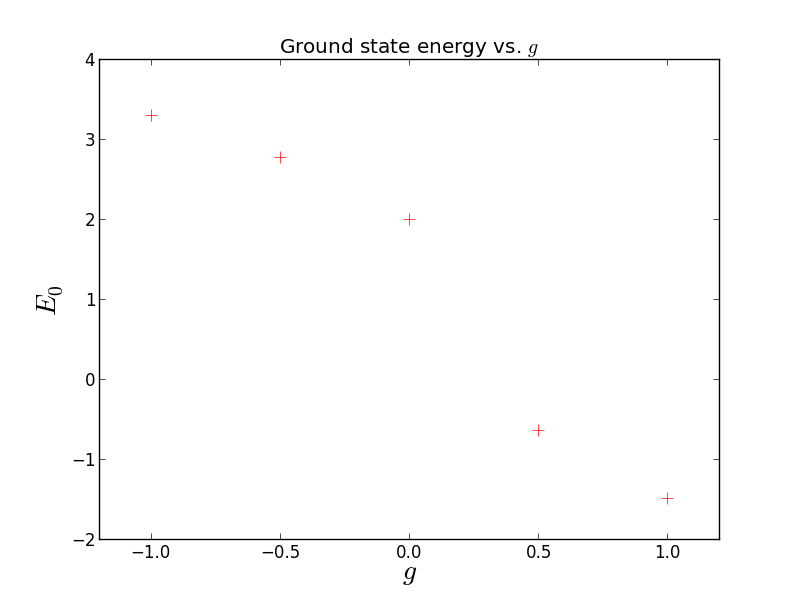
\includegraphics[width=0.6\textwidth]{lvl4pr2.png}
	\caption{Ground state energies for five different values of $g$ - calculated by diagonalizing the $6 \times 6$ Hamiltonian matrix of eq.~\ref{eq:ham6mtx}. These results match our code's output given in Table~\ref{tab:2pr4lvl}.}
	\label{fig:ezerovg}
\end{figure}



%Table~\ref{tab:1pr2lvl} lists the results of our shell model calculation with two particles (1 pair) and two levels.

\begin{table}[h]
\begin{center}
\begin{tabular}{|r|r|}
\hline
  g   &  $E_{gs}$ \\ \hline
-1.0  &  0.59 \\
-0.5  &  0.38 \\
 0.0  &  0.0 \\
 0.5  &  -0.62 \\
 1.0  &  -1.41 \\
\hline
\end{tabular}
\end{center}
\caption{Ground state energies as a function of interaction strength $g$ for the case of one pair in 2 single particle levels.}
\label{tab:1pr2lvl}
\end{table}


\begin{table}[h]
\begin{center}
	\begin{tabular}{|r|r|}
\hline
	g   &  $E_{gs}$ \\ \hline
	-1.0  &  3.30 \\
	-0.5  &  2.78 \\
	 0.0  &  2.0 \\
	 0.5  &  -0.64 \\
	 1.0  &  -1.49 \\
\hline
	\end{tabular}
\end{center}
	\caption{Ground state energies as a function of interaction strength $g$ for the case of two pairs in four levels.}
	\label{tab:2pr4lvl}
\end{table}





When we remove the single particle piece of the Hamiltonian and keep only
the two particle interaction, all particles are brought down to the same
degenerate energy level, with degeneracy $\Omega$ and ground state energy
\begin{equation}
	E_0 = - \frac{g}{4} n (\Omega - n +2)
	\label{eq:no1bdy}
\end{equation}

Our code reproduces the analytic result eq.~\ref{eq:no1bdy} for $g>0$ (an attractive two-body interaction). When 
$g$ becomes negative, eq.~\ref{eq:no1bdy} gives the highest possible energy level due to the two-body interaction
and the ground state energy becomes 0.

As we then vary the
interaction strength $g$ we observe the following pattern: In the
negative $g$ case, the interaction is repulsive, and so the best the
system can do is break even. In this case, the ground state energy is
zero, regardless of $g$. When $g$ becomes positive, however, the
interaction is attractive, and as $g$ becomes more and more positive,
the interaction becomes increasingly attractive and the system
correspondingly becomes more and more bound. We illustrate this for
several cases in Table \ref{tab:data-nosinglepart}.

%%% Tables
\begin{table}
\begin{center}
%\label{tab:data-nosinglepart}
\begin{tabular}{|c|c|c|c|}
\hline
   g   &  $E_{gs}$(2,2)  &  $E_{gs}$(6,6)  & $ E_{gs}$(8,8) \\ \hline
-1.0  &  0  &  0  &  0   \\
-0.5  &  0  &  0  &  0   \\
  0.0  &  0  &  0  &  0   \\
  0.5  &  -1  & -6  &  -10 \\
  1.0  &  -2  & -12 &  -20 \\
\hline
\end{tabular}
\end{center}
\caption{Ground state energies $E_{gs}(N_l,N_{part})$ for the case with
the single-particle Hamiltonian removed. The energies are shown as a
function of interaction strength $g$ for the case of $N_{part}$
particles in $N_l=\frac{\Omega}{2}$ single particle ``levels.''}
\label{tab:data-nosinglepart}
\end{table}

\clearpage

\definecolor{mygreen}{rgb}{0,0.6,0}
\definecolor{mygray}{rgb}{0.5,0.5,0.5}
\definecolor{mymauve}{rgb}{0.58,0,0.82}

\lstset{ %
  backgroundcolor=\color{white},   % choose the background color; you must add \usepackage{color} or \usepackage{xcolor}
  basicstyle=\footnotesize,        % the size of the fonts that are used for the code
  breakatwhitespace=false,         % sets if automatic breaks should only happen at whitespace
  breaklines=true,                 % sets automatic line breaking
  captionpos=b,                    % sets the caption-position to bottom
  commentstyle=\color{mygreen},    % comment style
  deletekeywords={...},            % if you want to delete keywords from the given language
  escapeinside={\%*}{*)},          % if you want to add LaTeX within your code
  extendedchars=true,              % lets you use non-ASCII characters; for 8-bits encodings only, does not work with UTF-8
  frame=single,	                   % adds a frame around the code
  keepspaces=true,                 % keeps spaces in text, useful for keeping indentation of code (possibly needs columns=flexible)
  keywordstyle=\color{blue},       % keyword style
  language=Octave,                 % the language of the code
  otherkeywords={*,...},           % if you want to add more keywords to the set
  numbers=left,                    % where to put the line-numbers; possible values are (none, left, right)
  numbersep=5pt,                   % how far the line-numbers are from the code
  numberstyle=\tiny\color{mygray}, % the style that is used for the line-numbers
  rulecolor=\color{black},         % if not set, the frame-color may be changed on line-breaks within not-black text (e.g. comments (green here))
  showspaces=false,                % show spaces everywhere adding particular underscores; it overrides 'showstringspaces'
  showstringspaces=false,          % underline spaces within strings only
  showtabs=false,                  % show tabs within strings adding particular underscores
  stepnumber=2,                    % the step between two line-numbers. If it's 1, each line will be numbered
  stringstyle=\color{mymauve},     % string literal style
  tabsize=2,	                   % sets default tabsize to 2 spaces
  title=\lstname                   % show the filename of files included with \lstinputlisting; also try caption instead of title
}

\lstinputlisting{shell_model.py}

%	&= \ppop{q} \left ( \commutatorexp{\pmop{s}}{\ppop{r}} \right ) \pmop{r} + \ppop{r} \left ( \commutatorexp{\ppop{q}}{\pmop{r}} \right ) \pmop{s}\\
%	&= \pcop{q} \left ( \commutatorexp{\paop{s}}{\pcop{r}} \right ) \paop{r} + \pcop{r} \left ( \commutatorexp{\pcop{q}}{\paop{r}} \right ) \paop{s}\\
%	&= \pcop{q} \paop{s} \pcop{r} \paop{r} - \pcop{q} \pcop{r} \paop{s} \paop{r}\\
%	& \hspace{4mm} + \pcop{r} \pcop{q} \paop{r} \paop{s} - \pcop{r} \paop{r} \pcop{q} \paop{s}\\

























\begin{comment}

%%% SIDE TRACK - UNNECESSARY %%%

\begin{equation}
	\commutator{\hop}{\sop{-}} = 2 \sum_{p}  \left ( (p-1) \cop{p}{-} \aop{p}{+} \right )
	\label{eq:hsminusres}
\end{equation}


We can now re-write the remaining terms in $ \left [ \hat{H}_0, \hat{S}^2 \right ]$.

\begin{align*}
	\commutator{\hop}{\sop{+}} \sop{-} &= 2 \sum _{pp'} (p-1) \cop{p}{+} \aop{p}{-} \cop{p'}{-} \aop{p'}{+}\\
	\sop{+} \commutator{\hop}{\sop{-}} &= 2 \sum _{pp'} (p'-1) \cop{p}{+} \aop{p}{-} \cop{p'}{-} \aop{p'}{+}\\
	\commutator{\hop}{\sop{-}} \sop{+} &= 2 \sum _{pp'} (p-1) \cop{p}{-} \aop{p}{+} \cop{p'}{+} \aop{p'}{-}\\
	\sop{-} \commutator{\hop}{\sop{+}} &= 2 \sum _{pp'} (p'-1) \cop{p}{-} \aop{p}{+} \cop{p'}{+} \aop{p'}{-}
\end{align*}

Taking \commutator{\hop}{\sop{+}} \sop{-}:

\begin{align*}
	\commutator{\hop}{\sop{+}} \sop{-} &= \sum _{pp'} (p-1) \cop{p}{+} \aop{p}{-} \cop{p'}{-} \aop{p'}{+}\\
	&= \sum _{pp'} (p-1) \cop{p}{+} \left ( \krondelt{p}{p'} -  \cop{p'}{-} \aop{p}{-} \right ) \aop{p'}{+}\\
	&= \sum _{pp'} (p-1) \left ( \krondelt{p}{p'} \cop{p}{+} \aop{p'}{+} -  \cop{p}{+} \cop{p'}{-} \aop{p}{-} \aop{p'}{+} \right )\\
	&= \sum _{pp'} (p-1) \left ( \krondelt{p}{p'} \cop{p}{+} \aop{p'}{+} -  \cop{p'}{-} \cop{p}{+} \aop{p'}{+} \aop{p}{-} \right )\\
	&= \sum _{pp'} (p-1) \left ( \krondelt{p}{p'} \cop{p}{+} \aop{p'}{+} -  \cop{p'}{-} \left ( \krondelt{p}{p'} - \aop{p'}{+} \cop{p}{+} \right ) \aop{p}{-} \right )\\
	&= \sum _{pp'} (p-1) \left ( \krondelt{p}{p'} \cop{p}{+} \aop{p'}{+} - \krondelt{p}{p'} \cop{p'}{-} \aop{p}{-} - \cop{p'}{-} \aop{p'}{+} \cop{p}{+} \aop{p}{-} \right )\\
	&= \sum _{p} (p-1) \cop{p}{+} \aop{p}{+} - \sum _{p} (p-1) \cop{p}{-} \aop{p}{-} - \sum _{pp'} (p-1) \cop{p'}{-} \aop{p'}{+} \cop{p}{+} \aop{p}{-}\\
	&= \sum _{p} (p-1) \numop{p}{+} - \sum _{p} (p-1) \numop{p}{-} - \sum _{pp'} (p-1) \cop{p'}{-} \aop{p'}{+} \cop{p}{+} \aop{p}{-}\\
\end{align*}

Taking \commutator{\hop}{\sop{-}} \sop{+}:

\begin{align*}
	\commutator{\hop}{\sop{-}} \sop{+} &= \sum _{pp'} (p-1) \cop{p}{-} \aop{p}{+} \cop{p'}{+} \aop{p'}{-}\\
	&= \sum _{pp'} (p-1) \cop{p}{-} \left ( \krondelt{p}{p'} - \cop{p'}{+} \aop{p}{+} \right ) \aop{p'}{-}\\
	&= \sum _{pp'} (p-1) \left ( \krondelt{p}{p'} \cop{p}{-} \aop{p'}{-} - \cop{p}{-} \cop{p'}{+} \aop{p}{+} \aop{p'}{-} \right )\\
	&= \sum _{pp'} (p-1) \left ( \krondelt{p}{p'} \cop{p}{-} \aop{p'}{-} -  \cop{p'}{+} \cop{p}{-} \aop{p'}{-} \aop{p}{+} \right )\\
	&= \sum _{pp'} (p-1) \left ( \krondelt{p}{p'} \cop{p}{-} \aop{p'}{-} -  \cop{p'}{+} \left ( \krondelt{p}{p'} - \aop{p'}{-} \cop{p}{-} \right ) \aop{p}{+} \right )\\
	&= \sum _{pp'} (p-1) \left ( \krondelt{p}{p'} \cop{p}{-} \aop{p'}{-} - \krondelt{p}{p'} \cop{p'}{+} \aop{p}{+} - \cop{p'}{+} \aop{p'}{-} \cop{p}{-} \aop{p}{+} \right )\\
	&= \sum _{p} (p-1) \cop{p}{-} \aop{p}{-} - \sum _{p} (p-1) \cop{p}{+} \aop{p}{+} - \sum _{pp'} (p-1) \cop{p'}{+} \aop{p'}{-} \cop{p}{-} \aop{p}{+}\\
	&= \sum _{p} (p-1) \numop{p}{-} - \sum _{p} (p-1) \numop{p}{+} - \sum _{pp'} (p-1) \cop{p'}{+} \aop{p'}{-} \cop{p}{-} \aop{p}{+}\\
\end{align*}

Plugging these results in for their respective terms in the the remnant of $ \left [ \hat{H}_0, \hat{S}^2 \right ]$:

\begin{align*}
	& \left [ \hat{H}_0, \hat{S}^2 \right ]\\
	&= \frac{1}{2} \left ( \commutator{\hop}{\sop{+}} \sop{-} + \sop{+} \commutator{\hop}{\sop{-}} + \commutator{\hop}{\sop{-}} \sop{+} + \sop{-} \commutator{\hop}{\sop{+}} \right )\\
	&= \sum _{p} (p-1) \numop{p}{+} - \sum _{p} (p-1) \numop{p}{-} - \sum _{pp'} (p-1) \cop{p'}{-} \aop{p'}{+} \cop{p}{+} \aop{p}{-}\\
	& + \sum _{pp'} (p'-1) \cop{p}{+} \aop{p}{-} \cop{p'}{-} \aop{p'}{+}\\
	& + \sum _{p} (p-1) \numop{p}{-} - \sum _{p} (p-1) \numop{p}{+} - \sum _{pp'} (p-1) \cop{p'}{+} \aop{p'}{-} \cop{p}{-} \aop{p}{+}\\
	& + \sum _{pp'} (p'-1) \cop{p}{-} \aop{p}{+} \cop{p'}{+} \aop{p'}{-}
\end{align*}





%%% ALTERNATIVE FOR [V,SS] = 0 %%%

Writing the term \sop{-} \commutator{\vop}{\sop{+}} explicitly:

\begin{align}
\begin{split}
	\sop{-} \commutator{\vop}{\sop{+}} &= \left ( \sminus{m} \right ) \left ( \twobody{q}{s} \right ) \left ( \splus{p} \right )\\
	& - \left ( \sminus{m'} \right ) \left ( \splus{p'} \right ) \left ( \twobody{q'}{s'} \right )
\end{split}
\label{eq:svs}
\end{align}

The first product of sums may be re-written as follows, noting that in \ref{eq:svsmk1} and \ref{eq:svsmk2} the first terms are dropped since \aop{s}{-} \aop{s}{-} and \cop{q}{+} \cop{q}{+} acting on any state will give 0.

\begin{align}
	& (-g) \sum_{m q s p} \cop{m}{-} \aop{m}{+} \cop{q}{+} \cop{q}{-} \aop{s}{-} \aop{s}{+} \cop{p}{+} \aop{p}{-}\\
	& (-g) \sum_{m q s p} \cop{m}{-} \aop{m}{+} \cop{q}{+} \cop{q}{-} \aop{s}{-} \left ( \krondelt{s}{p} -  \cop{p}{+} \aop{s}{+} \right ) \aop{p}{-}\\
	& (-g) \sum_{m q s p} \krondelt{s}{p} \cop{m}{-} \aop{m}{+} \cop{q}{+} \cop{q}{-} \aop{s}{-} \aop{p}{-} - \cop{m}{-} \aop{m}{+} \cop{q}{+} \cop{q}{-} \aop{s}{-}  \cop{p}{+} \aop{s}{+} \aop{p}{-}\\
\label{eq:svsmk1}	& (-g) \sum_{m q s p} \cop{m}{-} \aop{m}{+} \cop{q}{+} \cop{q}{-} \aop{s}{-} \aop{s}{-} - \cop{m}{-} \aop{m}{+} \cop{q}{+} \cop{q}{-} \aop{s}{-}  \cop{p}{+} \aop{s}{+} \aop{p}{-}\\
	& (-g) \sum_{m q s p}  - \cop{m}{-} \aop{m}{+} \cop{q}{+} \cop{q}{-} \aop{s}{-}  \cop{p}{+} \aop{s}{+} \aop{p}{-}\\
	& (-g) \sum_{m q s p}  \cop{m}{-} \aop{m}{+} \cop{p}{+} \cop{q}{+} \cop{q}{-} \aop{p}{-} \aop{s}{-} \aop{s}{+}\\
	& (-g) \sum_{m q s p}  \cop{m}{-} \aop{m}{+} \cop{p}{+} \cop{q}{+} \left ( \krondelt{q}{p} -  \aop{p}{-} \cop{q}{-} \right ) \aop{s}{-} \aop{s}{+}\\
	& (-g) \sum_{m q s p} \krondelt{q}{p} \cop{m}{-} \aop{m}{+} \cop{p}{+} \cop{q}{+} \aop{s}{-} \aop{s}{+} - \cop{m}{-} \aop{m}{+} \cop{p}{+} \cop{q}{+}  \aop{p}{-} \cop{q}{-} \aop{s}{-} \aop{s}{+}\\
\label{eq:svsmk2}	& (-g) \sum_{m q s p} \cop{m}{-} \aop{m}{+} \cop{q}{+} \cop{q}{+} \aop{s}{-} \aop{s}{+} - \cop{m}{+} \aop{m}{+} \cop{p}{+} \cop{q}{+}  \aop{p}{-} \cop{q}{-} \aop{s}{-} \aop{s}{+}\\
	& (-g) \sum_{m q s p} - \cop{m}{-} \aop{m}{+} \cop{p}{+} \cop{q}{+}  \aop{p}{-} \cop{q}{-} \aop{s}{-} \aop{s}{+}\\
	& (-g) \sum_{m q s p} - \cop{m}{-} \aop{m}{+} \aop{p}{-} \cop{p}{+} \cop{q}{+} \cop{q}{-} \aop{s}{-} \aop{s}{+}\\
\label{eq:svsmk3}	& (-g) \sum_{m q s p} \cop{m}{-} \aop{m}{+} \cop{p}{+} \aop{p}{-} \cop{q}{+} \cop{q}{-} \aop{s}{-} \aop{s}{+}
\end{align}

Comparing the result from \ref{eq:svsmk3} to the second product of sums in eq.~\ref{eq:svs} which we re-write here as

\begin{equation}
	g \sum _{m p qs} \cop{m}{-} \aop{m}{+} \cop{p}{+} \aop{p}{-} \cop{q}{+} \cop{q}{-} \aop{s}{-} \aop{s}{+} \nonumber
\end{equation}

we find that $ \sop{-} \commutator{\vop}{\sop{+}} =0$





\end{comment}

\end{document}